\chapter{Metapost}
\label{sec:mp}

前文提到Knuth的 \MF 可以用来设计矢量字体,但是输出的是点阵格式PK。1980年代末John D. Hobby\indexHobby{} \footnote{1985年斯坦福电脑博士,师从Knuth。后加入贝尔实验室。} 设计了一种绘图语言及其编译器,也就是 \MP ,它从 \MF 那里获得了大量灵感和源代码。

\MP 青出于蓝,它输出的是EPS,而且支持彩色;\MF 只支持黑白,因为它是用来设计字体的。\MP 可以在图形上加文字标注,甚至插入 \TeX 源码。同时它也从 \MF 那里继承了一些缺点:数值变量精度较低,且绝对值不能超过4096;只支持部分PostScript功能。雷人可以考虑用Asymptote取代 \MP。

1994年之后,Taco Hoekwater\indexHoekwater{} \footnote{曾学习艺术史和哲学,1992年辍学加入荷兰军队。退伍后加入克鲁沃学术出版公司 (Kluwer Academic Publishers) ,2000年跳槽到精灵公司 (Elvenkind)。LuaTeX和Con\TeX{}t的开发者之一。} 和Hagen等人接管了 \MP 的开发和维护工作。若想深入了解,可以参阅其用户手册\citep{Hobby_2010}。

\section{准备工作}

\MP 的缺省长度单位是bp,我们也可以使用 \autoref{tab:unit} 中的其它单位。也可以定义一个缩放系数,把坐标都转换为它的倍数,以后想缩放图形时只要修改这个系数即可。注意变量赋值符号是 \texttt{:=},而 \texttt{=} 则用于方程式。一个变量在同一源文件中只须定义一次,在其后的图形中都可以使用。

一个 \MP 源文件 (.mp) 可以包含多个图形,如 \autoref{exa:mp_src} 所示。代码中每行语句以分号结尾,注释以百分号起始。绘图命令包含在一对起始和结尾声明之间。文件结尾也要有一个结尾声明。

\begin{example}[h]
\begin{Code}[numbers=left]
u := 10pt;   %缩放系数
beginfig(1); %图形起始
...          %绘图命令
endfig;      %图形结尾

beginfig(2);
...
endfig;
...
end          %文件结尾
\end{Code}
\caption{\MP 源文件}
\label{exa:mp_src}
\end{example}

我们可以用命令行程序 \texttt{mpost}编译 \MP 源文件,生成一种特殊的EPS,也就是MPS;然后再把MPS插入 \LaTeX 源文件中使用。假设源文件名是 \texttt{fig.mp},可以执行以下编译命令,

\begin{Code}[]
mpost fig(.mp)
\end{Code}

编译后会得到“fig.1、fig.2、$\cdots$”等文件,每个文件的后缀就是相应的图形起始声明中的编号。此编号在一个源文件中应保持唯一,否则后生成的文件就会覆盖前面的。

数字文件名后缀不便于管理,\MP 为此提供了一个变量来设置输出文件名。我们可以把下面代码加到源文件头部,编译输出的文件名就会是“fig-01.mps、fig-02.mps、$\cdots$”;或者在在每个图形前面声明各自的名字。

\begin{Code}[]
outputtemplate "%j-%2c.mps";   %`加在源文件头部`
outputtemplate "flowchart.mps" %`加在每个图形前面`
\end{Code}

\texttt{xelatex} 不认识MPS格式,所以我们需要使用 \texttt{.eps} 后缀,或者用 \verb|\DeclareGraphicsRule| 命令把 \texttt{.mps} 声明为EPS。

\begin{Code}[]
\DeclareGraphicsRule{.mps}{eps}{.mps}{}
\end{Code}

\section{基本图形对象}

\subsection{点和直线}

\MP 的缺省画笔直径为0.5bp,拿它画点,直径就是0.5bp;拿它画线,宽度也是0.5bp。我们可以用 \texttt{withpen} 选项为单个绘图命令设置画笔,也可以用 \texttt{pickup} 命令为之后所有的绘图命令设置画笔。

在 \autoref{exa:mp_line} 中,\texttt{draw} 命令把几个点以直线段连接起来。\texttt{drawdot} 命令在指定坐标画点,为了使它醒目些我们可以换了支粗一点的画笔。

\begin{example}[h]
\begin{FBTDemo}[numbers=left]{\includegraphics{line.mps}}
filenametemplate "line.eps";
beginfig(1);
draw (0,0)--(4u,0)--(2u,2u)--(0,0) withpen pencircle scaled .8pt;
pickup pencircle scaled .8pt;
draw (5u,0)--(9u,0)--(7u,2u)--cycle;
pickup pencircle scaled 3pt;
drawdot (10u,0);
drawdot (14u,0);
drawdot (12u,2u);
endfig;
\end{FBTDemo}
\caption{\MP 点和直线}
\label{exa:mp_line}
\end{example}

几段直线或曲线可以构成一条路径 (path) ,在路径末尾加个 \texttt{cycle} 命令就构成封闭路径 (closed path) 。上例中两个三角形看起来都是封闭的,其实后面的才是真正的封闭路径。

\subsection{预定义形状}

 \texttt{fullcircle} 命令以原点为圆心画一个单位圆,类似的预定义形状还有 \texttt{halfcircle、quartercircle、unitsquare} 等。注意单位正方形的参考点在左下而不在其中心。在 \autoref{exa:mp_predefined} 中,我们使用了不同方向的缩放系数 \texttt{xscaled} 和 \texttt{yscaled},把把圆形和正方形变为椭圆和长方形。

\begin{example}[!h]
\begin{FBTDemo}[numbers=left]{\includegraphics{predefined.mps}}
filenametemplate "predefined.eps";
beginfig(3);
pickup pencircle scaled .8pt;
draw fullcircle scaled 2u;
draw halfcircle scaled 2u shifted (3u,0);
draw quartercircle scaled 2u shifted (5u,0);
draw fullcircle xscaled 4u yscaled 2u shifted (9u,0);
draw unitsquare scaled 2u shifted (12u,-u);
draw unitsquare xscaled 4u yscaled 2u shifted (15u,-u);
endfig;
\end{FBTDemo}
\caption{\MP 预定义形状}
\label{exa:mp_predefined}
\end{example}

\subsection{曲线}

如果把画直线时坐标点之间的 \texttt{--} 换成 \texttt{..},我们就得到一条曲线。直线和曲线共用一些点时,它们也可以混在一条语句里画。

\MP 的曲线用三次贝塞尔算法实现,我们还可以在曲线上使用方向 (direction) 、张力 (tension) 和曲率 (curl) 等控制。\autoref{exa:mp_curve} 中左列三图未加任何控制 (代码第四、七、十行) ,下排后两图使用了方向控制 (代码第五、六行) ,中排后两图使用了张力 (代码第八、九行) ,上排后两图使用了曲率 (代码第11、12行) 。

\begin{example}[h]
\begin{FBTDemo}[numbers=left]{\includegraphics{curve.mps}}
filenametemplate "curve.eps";
beginfig(3);
pickup pencircle scaled .8pt;
draw (0,0)..(4u,1u)..(8u,0);
draw (9u,0){up}..(13u,1u){right}..(17u,0){down};
draw (18u,0){up}...(22u,1u){right}...(26u,0){down};
draw (0,2u)..(2u,3u)..(6u,3u)..(8u,2u);
draw (9u,2u)..(11u,3u)..tension 1.5..(15u,3u)..(17u,2u);
draw (18u,2u)..(20u,3u)..tension 1.5 and 1..(24u,3u)..(26u,2u);
draw (0,4u)..(4u,5u)..(8u,4u);
draw (9u,4u){curl 0}..(13u,5u)..{curl 0}(17u,4u);
draw (18u,4u){curl 100}..(22u,5u)..{curl 100}(26u,4u);
pickup pencircle scaled 3pt;
drawdot (0,0); drawdot (4u,1u); drawdot (8u,0);
drawdot (9u,0); drawdot (13u,1u); drawdot (17u,0);
drawdot (18u,0); drawdot (22u,1u); drawdot (26u,0);
drawdot (0,2u); drawdot (2u,3u); drawdot (6u,3u); drawdot (8u,2u);
drawdot (9u,2u); drawdot (11u,3u); drawdot (15u,3u); drawdot (17u,2u);
drawdot (18u,2u); drawdot (20u,3u); drawdot (24u,3u); drawdot (26u,2u);
drawdot (0,4u); drawdot (4u,5u); drawdot (8u,4u);
drawdot (9u,4u); drawdot (13u,5u); drawdot (17u,4u);
drawdot (18u,4u); drawdot (22u,5u); drawdot (26u,4u);
\end{FBTDemo}
\caption{\MP 曲线}
\label{exa:mp_curve}
\end{example}

\section{图形控制}
\subsection{线型}

在绘制图形时,我们不仅可以变换线宽,也可以使用多种线型。

\begin{example}[h]
\begin{FBTDemo}[numbers=left]{\includegraphics{dashed.mps}}
filenametemplate "dashed.eps";
beginfig(4);
pickup pencircle scaled .8pt;
draw (0,0)--(10u,0) dashed withdots;
draw (0,1u)--(10u,1u) dashed withdots scaled 2;
draw (0,2u)--(10u,2u) dashed evenly;
draw (0,3u)--(10u,3u) dashed evenly scaled 2;
endfig;
\end{FBTDemo}
\caption{\MP 线型}
\label{exa:mp_dashed}
\end{example}

\subsection{箭头}

箭头画法如下,注意反向箭头需要把两个坐标用一对圆括号括起来。

\begin{example}[!h]
\begin{FBTDemo}[numbers=left]{\includegraphics{arrow.mps}}
filenametemplate "arrow.eps";
beginfig(5);
pickup pencircle scaled .8pt;
drawarrow (0,0)--(10u,0);
drawarrow reverse ((0,1u)--(10u,1u));
drawdblarrow (0,2u)--(10u,2u);
endfig;
\end{FBTDemo}
\caption{\MP 箭头}
\label{exa:mp_arrow}
\end{example}

\subsection{彩色和填充}

\MP 不能使用 \texttt{xcolor} 宏包,它只支持rgb和cmyk色彩模式,预定义了黑、白、红、绿、蓝等颜色。自定义颜色的方法如下,

\begin{Code}[]
color c[];
c1 := .9red + .6green + .3blue;
c2 := (.9,.6,.3);
\end{Code}

绘图命令一般可以通过 \texttt{withcolor} 选项来使用各种颜色。

\begin{example}[h]
\begin{FBTDemo}[numbers=left]{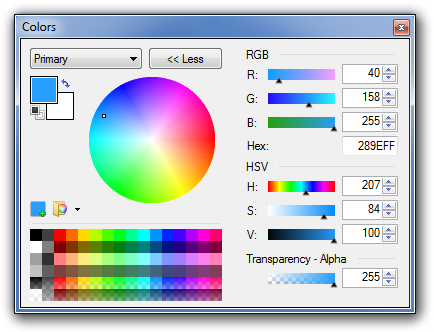
\includegraphics{color.mps}}
filenametemplate "color.eps";
beginfig(6);
pickup pencircle scaled .8pt;
draw (0,0)--(10u,0) withcolor red;
draw (0,1u)--(10u,1u) withcolor green;
draw (0,2u)--(10u,2u) withcolor blue;
endfig;
\end{FBTDemo}
\caption{\MP 彩色}
\label{exa:mp_color}
\end{example}

封闭路径可以用 \texttt{fill} 命令来填充。\autoref{exa:mp_fill} 中第三、四行代码定义了一个 \texttt{path} 变量,以便后面重用。另一个命令 \texttt{filldraw} 可以看作是 \texttt{fill+draw},它除了填充外还会把路径用指定的画笔画一遍。然而不幸的是画边缘和填充内部只能用同一种颜色,所以它的用处不大。

\begin{example}[h]
\begin{FBTDemo}[numbers=left]{\includegraphics{fill.mps}}
filenametemplate "fill.eps";
beginfig(7)
path p;
p := (0,0)--(2,0)--(1,1.732)--cycle;
fill p scaled u;
fill p scaled u shifted (3u,0) withcolor red;
fill p scaled u shifted (6u,0) withcolor green;
fill p scaled u shifted (9u,0) withcolor blue;
endfig;
\end{FBTDemo}
\caption{\MP 填充}
\label{exa:mp_fill}
\end{example}

除了为每个绘图命令单独指定颜色,我们也可以使用一个全局命令 \texttt{drawoption},使得其后的绘图命令都使用某种颜色。

\begin{Code}[]
drawoption(withcolor blue);
\end{Code}

\section{图形变换}

除了前文提到的缩放,我们还可以对路径进行平移 (\texttt{shifted}) 、旋转 (\texttt{rotated}) 、定点旋转 (\texttt{rotatedaround}) 、镜像 (\texttt{reflectedabout})  、倾斜 (\texttt{slanted})等变换操作。平移的参数是移到的坐标点;旋转的参数是角度,旋转中心是原点;定点旋转的参数是旋转中心;倾斜的参数是倾斜比;镜像的参数是两点确定的一条直线。

这些变换操作可以任意结合使用。由于旋转是围绕原点进行的,所以要注意平移和旋转的顺序。\autoref{exa:mp_transform} 中重用了 \autoref{exa:mp_fill} 中定义的路径。

\begin{example}[h]
\begin{FBTDemo}[numbers=left]{\includegraphics{transform.mps}}
filenametemplate "transform.eps";
beginfig(8);
pickup pencircle scaled .8pt;
draw p scaled u;
draw p scaled u shifted (3u,0) rotated 30;
draw p scaled u rotated 30 shifted (5u,0);
draw p scaled u rotatedaround ((2u,0),30) shifted (7u,0) ;
draw p scaled u slanted 1 shifted (10u,0);
draw p scaled u reflectedabout ((0,0),(2u,0)) shifted (13u,0);
draw p xscaled 2u yscaled u shifted (16u,0);
endfig;
\end{FBTDemo}
\caption{\MP 图形变换}
\label{exa:mp_transform}
\end{example}

\section{标注}

 \texttt{label} 命令可以在指定位置加文字标注,该命令有八种后缀,对应着指定坐标点的八个方位 (见 \autoref{tab:mp_label}) 。\texttt{dotlabel} 命令在加标注同时画了个点,它也用同样的方法表示标注的方位。

\begin{table}[htbp]
\centering
\caption{ \texttt{label} 命令的方位}
\label{tab:mp_label}
\begin{tabular}{llllllll}
    \toprule
    top  & 上   & bottom & 下   & lft  & 左   & rt  & 右 \\
    ulft & 左上 & urt    & 右上 & llft & 左下 & lrt & 右下 \\
    \bottomrule
\end{tabular}
\end{table}

我们也可以用一对 \texttt{btex} 和 \texttt{etex} 来嵌入一些 \TeX 内容,比如数学标注 (\autoref{exa:mp_label} 代码第14、18、19行) 。\texttt{mpost} 会把 \TeX 内容存到一个临时文件,调用 \texttt{tex} 编译它生成DVI; \texttt{mpost} 把DVI转换为\MP 内容存到一个 \texttt{.mpx} 文件中,然后再把它嵌入输出的MPS。

\begin{example}[h]
\begin{FBTDemo}[numbers=left]{\includegraphics{label.mps}}
prologues:=3;
filenametemplate "label.eps";
beginfig(9);
pickup pencircle scaled .8pt;
draw unitsquare xscaled 8u yscaled 4u;
label.top ("top", (4u,4u));
label.bot ("bottom", (4u,0));
label.lft ("left", (0,2u));
label.rt ("right", (8u,2u));
label.ulft ("upper left", (0,4u));
label.urt ("upper right", (8u,4u));
label.llft ("lower left", (0,0));
label.lrt ("lower right", (8u,0));
label.rt (btex $E=mc^2$ etex, (2u,2u));
drawarrow (16u,0)--(22u,0);
drawarrow (16u,0)--(16u,4u);
dotlabel.bot ("(0,0)", (16u,0));
label.bot (btex $x$ etex, (22u,0));
label.lft (btex $y$ etex, (16u,4u));
endfig;
\end{FBTDemo}
\caption{\MP 标注}
\label{exa:mp_label}
\end{example}

\MP 中也可以嵌入复杂的 \LaTeX 代码,比如字体和语言等的设置。这时需要在源文件头尾加两对 \texttt{verbatimtex} 和 \texttt{etex} 命令,分别包含前置和后置处理代码,原图形代码放在这两对命令之间。可惜\MP 不支持嵌入 \XeLaTeX 代码,所以其文字标注不能使用后者的字体功能。

MPS缺省不嵌入字体,当它包含文字时,GSview就不能正常查看;但是把这种MPS插入文档生成的PDF还是正常的,因为驱动会自行处理字体。我们可以强制MPS嵌入字体,一种方法是在源文件头部加一行语句 (\autoref{exa:mp_label} 代码第一行) ,另一种方法是在编译时加一个参数,

\begin{Code}[]
mpost \prologues:=3; input fig.mp
\end{Code}

\section{编程}
\subsection{数据类型和变量}

\MP 中有十种基本数据类型:\texttt{numeric、pair、path、pen、color、cmykcolor、transform、string、boolean、picture}。我们已经接触过其中几种,比如缩放系数 \texttt{u} 是 \texttt{numeric},点的坐标是 \texttt{pair},几个点用直线连起来是一个 \texttt{path},\texttt{pencircle} 是一种 \texttt{pen},红、绿、蓝都是 \texttt{color},\texttt{scaled、shifted、rotated} 都是 \texttt{transform}。

numeric类型变量的精度是1/65536,它的绝对值不能超过4096,在计算过程中数值可以达到32768。这样的规定也应归功于当年的电脑硬件,不过对于科技文档插图而言,4096一般还是够用的。

除了缺省的numeric,其它变量在使用之前都需要用数据类型来显式声明。相同类型的变量可以在一行语句中声明,但是带下标的变量不能放在同一行 (这个规定很蹊跷) 。

\begin{Code}
numeric x,y,z;    %正确
numeric x1,x2,x3; %错误
numeric x[];      %正确
\end{Code}

\subsection{数学运算}

\MP 中可以使用普通的运算符,比如 \verb|+ - * /|;也提供一些特殊的运算符,比如\verb|a++b| 表示$\sqrt{a^2+b^2}$,\verb|a+-+b| 表示$\sqrt{a^2-b^2}$;另外 \autoref{tab:mp_math_func} 列出一些常用数学函数。

\begin{table}[htbp]
\centering
\caption{\MP 数学函数}
\label{tab:mp_math_func}
\begin{tabular}{llll}
    \toprule
    \texttt{abs}     & 绝对值   & \texttt{mexp} & 指数 \\
    \texttt{round}   & 四舍五入 & \texttt{mlog} & 对数 \\
    \texttt{ceiling} & 向上圆整 & \texttt{sind} & 正弦 \\
    \texttt{floor}   & 向下圆整 & \texttt{cosd} & 余弦 \\
    \texttt{mod}     & 模余     & \texttt{normaldeviate} & 正态分布随机数 \\
    \texttt{sqrt}    & 开方     & \texttt{uniformdeviate} & 均匀分布随机数 \\
    \bottomrule
\end{tabular}
\end{table}

\subsection{循环}

当执行重复任务时,循环语句可以让程序变得简洁 (见 \autoref{exa:mp_loop}) 。

\begin{example}[h]
\begin{FBTDemo}[numbers=left]{\includegraphics{loop.mps}}
filenametemplate "loop.eps";
beginfig(10);
pickup pencircle scaled .8pt;
drawarrow (0,0)--(10u,0);
drawarrow (0,0)--(0,4u);
draw (0,0) %注意这里没有分号
for x=1 upto 3: ..(x*x,x)*u endfor;
endfig;
\end{FBTDemo}
\caption{\MP 循环}
\label{exa:mp_loop}
\end{example}

循环语句缺省步长是1,我们也可以改用其它步长。\texttt{upto} 其实就是 \texttt{step 1 until} 的简写方式。

\begin{Code}[]
for x=1 step .5 until 3: 
\end{Code}

\bibliographystyle{unsrtnat}
\bibliography{lnotes2}
